%
% ────────────────────────────────────────────────────────────────────────── I ──────────
%   :::::: C A D E N A S   D E   M A R K O V : :  :   :    :     :        :          :
% ────────────────────────────────────────────────────────────────────────────────────
%

Hasta este momento, en los dos primeros capítulos, nos hemos centrado totalmente en una introducción teórico-práctica a los polinomios ortogonales y sus principales propiedades, profundizando en las llamadas familias clásicas. En este capítulo explicaremos una teoría probabilística que, aparentemente, nada tiene que ver con los polinomios ortogonales, aunque estudiaremos la estrecha relación que hay entre ambas teorías en el capítulo \ref{chap:POyPNM}.

En concreto, analizaremos desde un punto de vista general los llamados \textit{procesos de Markov, procesos markovianos} o simplemente \textit{cadenas de Markov}. Estos modelos, basados en estados, tratan de explicar las probabilidades de los posibles cambios de estado de un sistema a partir de  un principio denominado \textit{propiedad de Markov}. Esta denominación tanto del modelo como de la propiedad se debe a \textsc{Andrey Markov}, matemático que fue el primero en estudiar, en la década de 1900, los procesos estocásticos con dicha propiedad, que posteriormente se popularizarían.

Nos centraremos principalmente en procesos discretos, es decir, consideramos que el tiempo se divide en instantes $n=0,1,2,\dots$, sin olvidar que existe una formulación análoga en la que el tiempo es continuo $t\in[0,\infty)$. Denominamos \textit{estado} a cualquiera de las situaciones en las que se puede encontrar el sistema en un instante determinado. Por ejemplo, pensemos en un barrio en el que hay $N$ fruterías y dividimos el tiempo en semanas. Asumimos que un individuo siempre va a comprar a una de estas tiendas aunque hay posibilidad de que cambie de una a otra distinta cada semana. Etiquetamos cada una de las fruterías con un número: frutería $1$, frutería $2$,\dots, frutería $N$.

\section{Cadenas de Markov discretas. Matriz de transición}

De forma general, consideramos un espacio de estados finito que con frecuencia denotaremos como $S=\{1,\dots, N\}$ y dividimos el tiempo en instantes $n=0,1,2,\dots$. Llamemos $X_n\in S$ al estado del sistema en el instante $n$. La propiedad específica que consideró Markov consiste en asumir que, suponiendo que el sistema se encuentra en un estado concreto en un instante concreto, la probabilidad de que ocurra una transición en el siguiente instante depende única y exclusivamente del estado actual.

\begin{definicion}[Cadena de Markov]
    Un proceso estocástico $\{X_n,n\geq 0\}$ en un espacio de estados $S$ verifica la \textbf{propiedad markoviana} o \textbf{propiedad de Markov} si, para todo $n\in\N_0$ y $j,i,i_{n-1},\dots, i_0 \in S$:
    \begin{equation}
        \label{eq:prop-markow}
        P[X_{n+1}=j | X_n=i, X_{n-1}=i_{n-1}, \dots, X_0=i_0 ] = P[X_{n+1}=j | X_n=i].
    \end{equation}

    En caso de que el proceso cumpla la propiedad (\ref{eq:prop-markow}) se denominará \textbf{cadena de Markov discreta}.

    Una cadena de Markov $\{X_n, n\geq 0\}$ se llamará \textbf{homogénea} si, para todo $n\in\N_0$,
    \begin{equation}
        \label{eq:cad-homogenea}
        P[X_{n+1}=j|X_n=i] = P[X_1=j|X_0=i].
    \end{equation}
\end{definicion}

Es decir, la probabilidad de que en un instante $n+1$ el sistema se encuentre en el estado $j$ es independiente de lo que haya ocurrido en los instantes anteriores a $n$. Por ejemplo, aplicando esta propiedad al tiempo atmosférico podríamos afirmar que la probabilidad de que mañana llueva únicamente depende de si hoy ha llovido, sin tener en cuenta el clima de los días anteriores. En epidemiología, es como afirmar que el número de contagios de una enfermedad un día concreto puede predecirse a partir del número de contagios que haya habido el día anterior, independientemente del número de contagios de los días anteriores ni los posibles factores externos. Intuitivamente, no parece que esta suposición sea muy realista y no cabe esperar resultados precisos en predicciones futuras. Sin embargo, lo cierto es que es útil para hacernos una idea de lo que puede ocurrir a largo plazo con relativa exactitud y es muy utilizada a la hora de implementar medidas en ámbitos como la migración, la extinción de animales, uso de suelo, etc.

La probabilidad $P[X_{n+1}=j|X_n=i]$ se denomina \textbf{probabilidad de transición en un paso} de la cadena en el instante $n$. Si además la cadena es homogénea, este valor es el mismo para todo instante $n$, de ahí el término `homogénea'. En adelante, cuando utilicemos el término `cadena de Markov' nos estaremos refiriendo a una cadena de Markov homogénea. Una vez anulada la dependencia de $n$, introducimos una nueva notación:
$$
p_{ij} := P[X_{n+1}=j|X_n=i], \ \ \forall i,j \in \{1,\dots,N\}.
$$
Con esta notación, y teniendo en cuenta que en un espacio de $N$ estados existen $N^2$ posibles transiciones, agrupamos todas estas probabilidades en una matriz.

\begin{definicion}[Matriz de transición]
    Llamamos \textbf{matriz de transición} de una cadena de Markov $\{X_n, n\geq 0\}$ a la matriz
    \begin{equation}
        \label{eq:matriz-trans}
        P=\begin{pmatrix}
          p_{11} & p_{12} & \cdots & p_{1N} \\
          p_{21} & p_{22} & \cdots & p_{2N} \\
          \vdots & \vdots & \ddots & \vdots \\
          p_{N1} & p_{N2} & \cdots & p_{NN}  
        \end{pmatrix}.
    \end{equation}
\end{definicion}

\begin{observacion}
    Obsérvese que la $i$-ésima fila corresponde a la distribución de la probabilidad saliente del estado $i$, mientras que la $j$-ésima columna describe la probabilidad entrante al estado $j$.
\end{observacion}

Presentamos a continuación dos propiedades directas de las matrices de transición.

\begin{proposicion}
    \label{prop:propiedades-matrices-markov}
Sea $\{X_n, n\geq 0\}$ una cadena de Markov sobre el espacio de estados $S=\{1,\dots,N\}$ y cuya matriz de transición es $P=(p_{ij})_{i,j=1,\dots,N}$. Entonces
\begin{enumerate}
    \item $0\leq p_{ij} \leq 1 \ \ \ \forall i,j\in S$.
    \item $\sum_{j=1}^N p_{ij} = 1 \ \ \ \forall i\in S$ (todas las filas de $P$ suman 1).
\end{enumerate}
\end{proposicion}
\begin{proof}
    La propiedad (1) es evidente teniendo en cuenta que $p_{ij}$ es una probabilidad. Sobre la propiedad (2), tenemos que
    \begin{equation*}
        \begin{split}
            \sum_{j=1}^N p_{ij} &= \sum_{j=1}^N P[X_{n+1}=j|X_n=i] \\
            &= P[X_{n+1}\in S|X_n=i] \ \ \text{(por el teorema de la probabilidad total)} \\
            &= 1
        \end{split}
    \end{equation*}
\end{proof}

A las matrices que cumplen estas dos propiedades se les denomina \textbf{matrices estocásticas} y pueden ser consideradas matrices de transición de alguna cadena de Markov.

\begin{ejemplo}[Tiempo atmosférico]
    \label{ej:tiempo}
    Extraído de \cite[Ch. 2, Example 2.3]{kulkarni-2012}. Supongamos que podemos clasificar el tiempo de una ciudad como soleado (1), nublado (2) o lluvioso (3) y que el tiempo del día siguiente únicamente depende del tiempo del día anterior con las siguientes probabilidades:
    \begin{itemize}
        \item Si hoy hace sol, mañana estará nublado con probabilidad $0.3$ y lloverá con probabilidad $0.2$.
        \item Si hoy está nublado, mañana hará sol con probabilidad $0.5$ y lloverá con probabilidad $0.3$.
        \item Si hoy está lloviendo, mañana será un día soleado con probabilidad $0.4$ y nublado con probabilidad $0.5$.
    \end{itemize}

    Modelaremos este sistema mediante una cadena de Markov. Para ello, consideraremos la variable $X_n \equiv$ ``Tiempo atmosférico en el día $n$''. Y consideramos el espacio de estados $S = \{ 1\equiv\text{soleado}, 2\equiv\text{nublado}, 3\equiv\text{lluvioso}\}$. Atendiendo a las indicaciones anteriores y al item (2) de la proposición \ref{prop:propiedades-matrices-markov}, la matriz de transición sería por tanto
    $$ P = \begin{pmatrix}
        0.5 & 0.3 & 0.2 \\
        0.5 & 0.2 & 0.3 \\
        0.4 & 0.5 & 0.1
    \end{pmatrix}.
    $$

\end{ejemplo}

\section{Distribuciones transitorias}

Hasta el momento nos hemos centrado en la adaptación de distintas situaciones de acuerdo a modelos de estados regidos por cadenas de Markov, que en el caso homogéneo concentra toda su información en una matriz estocástica que denominamos matriz de transición. Sin embargo, ya adelantamos en la introducción que la principal función de este método consiste en tratar de predecir el comportamiento de la variable $X_n$ en algún instante futuro. Pongamos el caso del ejemplo \ref{ej:tiempo} sobre el tiempo atmosférico. Podría interesar predecir el tiempo que va a hacer dentro de 2 o 3 días para posponer o no un evento por lluvia. En esta sección estudiaremos cómo podemos utilizar cadenas de Markov con este objetivo.

Sea $\{X_n, n\geq 0\}$ una cadena de Markov discreta y homogénea sobre un espacio de estados $S=\{1,\dots,N\}$, una matriz de transición $P$ y supongamos conocida la distribución inicial, que denotaremos en forma de vector fila como $a^{(0)} = (a_1, \dots, a_N)$, donde $a_i = P[X_0 = i]$, $\forall i \in S$. Se denomina \textbf{distribución transitoria} a la distribución que sigue la variable $X_n$ para cierto $n\geq 0$ fijo cuando es conocida la distribución de $X_0$.

Abordemos este problema con lo que conocemos hasta el momento. Tenemos que
\begin{equation}
    \label{eq:distr-trans}
    \begin{split}
        P[X_n = j] &= \sum_{i=1}^N P[X_n=j|X_0 = i]P[X_0=i] \\
        &= \sum_{i=1}^Na_i \, P[X_n=j|X_0 = i].
    \end{split}
\end{equation}

Por lo que nuestro problema se reduce a encontrar la probabilidad de que el proceso esté en el estado $j$ tras $n$ instantes suponiendo que inicialmente se encontraba en el estado $i$, $P[X_n=j|X_0 = i]$. Esta probabilidad extiende a la que en su momento llamamos probabilidad de transición en un paso y, naturalmente, se denomina \textbf{probabilidad de transición en }$\mathbf{n}$ \textbf{pasos}. Utilizamos la notación  
\begin{align*}
    a_i^{(n)} &:= P[X_n=i], & p_{ij}^{(n)} &:= P[X_{n}=j|X_0=i],
\end{align*}
$\forall i,j \in \{1,\dots,N\}$. De esta forma, estamos denotando la función masa de probabilidad (a menudo abreviada como ``fmp'') de la variable aleatoria $X_n$ mediante el vector $a^{(n)}=(a_1^{(n)},\dots,a_N^{(n)})$. Recordemos que la fmp de una variable aleatoria discreta determina unívocamente su distribución, por lo cual en adelante utilizaremos indistintamente el término `distribución' y `función masa de probabilidad', sin olvidar que en realidad son conceptos distintos. 

Análogamente al caso en el que considerábamos un único paso, agrupamos todos los posibles valores de $p_{ij}^{(n)}$ en una matriz.

\begin{definicion}[Matriz de transición en $n$ pasos]
    Llamamos \textbf{matriz de transición en }$\mathbf{n}$ \textbf{pasos} de una cadena de Markov $\{X_n, n\geq 0\}$ a la matriz
    \begin{equation}
        \label{eq:matriz-trans-n}
        P^{(n)}=\begin{pmatrix}
          p_{11}^{(n)} & p_{12}^{(n)} & \cdots & p_{1N}^{(n)} \\
          p_{21}^{(n)} & p_{22}^{(n)} & \cdots & p_{2N}^{(n)} \\
          \vdots & \vdots & \ddots & \vdots \\
          p_{N1}^{(n)} & p_{N2}^{(n)} & \cdots & p_{NN}^{(n)}  
        \end{pmatrix}.
    \end{equation}
\end{definicion}

\begin{observacion}
    Si tomamos $n=0$, tenemos que $p_{ij}=\delta_{ij}$, $i,j\in S$. Esto es, $P^{(0)}=I_N$. Por otro lado, si $n=1$, tenemos que $P^{(1)}=P$, la matriz de transición (\ref{eq:matriz-trans}).
\end{observacion}

A partir de la definición de matriz de transición en $n$ pasos podemos reescribir (\ref{eq:distr-trans}) de forma matricial como
$$
a^{(n)}= a^{(0)} \cdot P^{(n)}.
$$

Por lo que resta obtener un método para calcular la matriz de transición en $n$ pasos, $P^{(n)}$. Este método nos lo da el siguiente teorema:

\begin{teorema}[Matriz de transición en $n$ pasos]
    \label{th:matriz-trans-n}
    Sea $\{X_n,n\geq 0\}$ una cadena de Markov homogénea con matriz de transición $P$, entonces
    \begin{equation}
        \label{eq:matriz-trans-n-teorema}
        P^{(n)} = P^n.
    \end{equation}    
\end{teorema}
\begin{proof}
    Consúltese \cite[Ch. II, theorem 2.2]{kulkarni-2012}.
\end{proof}

De este resultado obtenemos dos sencillas consecuencias:

\begin{corolario}
    \label{cor:fmp}
    La variable aleatoria $X_n$ se distribuye según la función masa de probabilidad descrita por el vector 
    $$
    a^{(n)} = a^{(0)}\cdot P^n.
    $$
\end{corolario}

Y aplicando la homogeneidad que asumimos en toda cadena:

\begin{corolario}
    \label{cor:Pnm}
    $$
    P[X_{n+m}=j|X_n=i,X_{n-1}=i_{n-1},\dots,X_0=i_0] = P[X_{n+m}=j|X_n=i]=p_{ij}^{(m)},
    $$
$j,i,i_{n-1},\dots,i_0\in S$.
\end{corolario}

Seguidamente, presentamos una ecuación importante en este ámbito.

\begin{teorema}[Ecuación de Chapman-Kolmogorov]
    Sea $\{X_n,n\geq 0\}$ una cadena de Markov discreta y homogénea, entonces las probabilidades de transición en $n$ pasos satisfacen la siguiente igualdad, denominada ecuación de Chapman-Kolmogorov.
    \begin{equation}
        \label{eq:chapman-kolmogorov}
        p_{ij}^{(n+m)}=\sum_{k=1}^N p_{ik}^{(n)}p_{kj}^{(m)}.
    \end{equation} 
\end{teorema}
\begin{proof}
    \begin{equation*}
        \begin{split}
            p_{ij}^{(n+m)} &= P[X_{n+m}=j|X_0=i] \\
            &= \sum_{k=1}^N P[X_{n+m}=j|X_n=k,X_0=i]\,P[X_n=k|X_0=i]\text{ (th. de la prob. total)}\\
            &= \sum_{k=1}^N P[X_{n+m}=j|X_n=k]\,P[X_n=k|X_0=i]\text{ (corolario \ref{cor:Pnm})}\\
            &= \sum_{k=1}^N P[X_{m}=j|X_0=k]\,P[X_n=k|X_0=i]\text{ (por la homogeneidad)}\\
            &= \sum_{k=1}^N p_{ik}^{(n)} p_{kj}^{(m)}
        \end{split}
    \end{equation*}
\end{proof}

Si escribimos la ecuación (\ref{eq:chapman-kolmogorov}) en forma matricial, tenemos que
$$
P^{(n+m)}=P^{(n)}\cdot P^{(m)},
$$
lo cual es evidente teniendo en cuenta el teorema \ref{th:matriz-trans-n}. Intercambiando los roles de $n$ y $m$ llegamos a la conclusión de que las matrices $P^{(n)}$ y $P^{(m)}$ conmutan para todo $n,m\geq 0$. El teorema \ref{th:matriz-trans-n} es la clave del método para calcular las distribuciones transitorias, pues reduce el problema a potencias y multiplicaciones de matrices.

\begin{ejemplo}\label{ej:cv}
    Tratemos ahora un ejemplo distinto. En este caso nos centraremos en las variaciones interprovinciales. La tabla \ref{tab:variaciones} muestra en cada celda el número de individuos que cambiaron su vivienda habitual desde la provincia indicada en la fila hacia la provincia indicada en la columna correspondiente (datos extraídos del INE: Instituto Nacional de Estadística).

    \begin{table}[h]
        \centering
        \begin{tabular}{cccc}\hline
            \textbf{Provincia} & \textbf{Alicante} & \textbf{Castellón} & \textbf{Valencia} \\ \hline\hline
        \textbf{Alicante}                  & 41.685                    & 484                         & 3.957                      \\ \hline
        \textbf{Castellón}                & 369                       & 11.059                      & 2.232                      \\ \hline
        \textbf{Valencia}                & 3.516                     & 2.903                       & 71.741 \\ \hline            
        \end{tabular}
        \caption{Variaciones interprovinciales en la comunidad valenciana (2021)}
        \label{tab:variaciones}
        \end{table}

        % https://www.ine.es/jaxi/Datos.htm?tpx=53144#!tabs-tabla
        % https://www.ine.es/jaxiT3/Datos.htm?t=2852

        Por su parte, la tabla \ref{tab:poblacion} muestra la población de cada una de las provincias en el año 2021. 

        \begin{table}[h]
            \centering
            \begin{tabular}{cc}\hline
                \textbf{Provincia}  & \textbf{Población} \\ \hline\hline
                \textbf{Alicante} &  1881762 \\ \hline
                \textbf{Castellón} & 587064 \\ \hline
                \textbf{Valencia} & 2589312 \\ \hline
            \end{tabular}
            \caption{Población de las provincias de la comunidad valenciana (2021)}
            \label{tab:poblacion}
        \end{table}

        Con estos datos y asumiendo que la población total permanece constante, ¿podemos comprobar la población de cada una de las provincias de la Comunidad Valenciana en el año 2022? ¿Y predecir las que habrá en el año 2023?

        Antes de proceder al propio modelado, queremos mencionar que estos datos han sido manipulados y presentados utilizando el software estadístico \texttt{R}\footnote{Consúltese su página web \url{https://www.r-project.org/}.}. El archivo de `R Markdown' \texttt{software/ejemplo-migraciones.Rmd} 
        contiene el código fuente en \texttt{R} y algunas descripciones, mientras que el fichero \texttt{software/ejemplo-migraciones.html}, aunque tiene el mismo contenido, es un archivo compilado que es posible abrir con cualquier navegador web y en el que no es necesario ejecutar nada para visualizar las salidas de los distintos comandos\footnote{Ambos ficheros están disponibles en las URLs \url{https://github.com/JAntonioVR/Polinomios-Ortogonales/blob/main/software/ejemplo-migraciones.Rmd} y \url{https://github.com/JAntonioVR/Polinomios-Ortogonales/blob/main/software/ejemplo-migraciones.html}}. 

        Procedemos a modelar el problema como una cadena de Markov $\{X_n,n\geq0\}$, donde 
        $$X_n \equiv \text{Provincia en la que reside un individuo al azar de la C. Valenciana en }2021+n.$$ 
        Esta cadena se construye sobre los estados 
        $$
        S=\{1\equiv\text{`Alicante'}, 2\equiv\text{`Castellón'},3\equiv\text{`Valencia'}\}.
        $$
        Podemos tomar una matriz asociada a la tabla \ref{tab:variaciones} y a partir de ella construir la matriz de transición de la cadena, teniendo en cuenta que de esta matriz la celda $(i,j)$ representa el número de migraciones de la provincia $i$ a la provincia $j$. Sin embargo, es claro que la tabla \ref{tab:variaciones} no verifica las condiciones de la proposición \ref{prop:propiedades-matrices-markov}, por lo que no podemos formar directamente una matriz estocástica. De igual manera, el vector cuyas componentes son las de la tabla \ref{tab:poblacion} no puede denotar una función masa de probabilidad pues sus componentes no suman $1$. Por suerte, estos problemas pueden solucionarse rápidamente sin más que dividir cada fila de la tabla \ref{tab:variaciones} entre el total de cada fila y cada componente de la tabla \ref{tab:poblacion} entre la suma de las tres celdas. De esta forma, tenemos la siguiente matriz de transición $P$ y la distribución inicial $a^{(0)}$.
        \begin{equation*}
            \label{eq:ejemplo-migraciones-matriz}
            P = \begin{pmatrix}
                0.90372024 & 0.01049300 & 0.08578676 \\
                0.02701318 & 0.80959004 & 0.16339678 \\
                0.04498465 & 0.03714176 & 0.91787359
            \end{pmatrix}, 
        \end{equation*}
        \begin{equation*}
            a^{(0)} = \begin{pmatrix}
                0.3720266 &
                0.1160633 &
                0.5119101
            \end{pmatrix}.
        \end{equation*}
         
        
        Por tanto, para conocer la distribución poblacional del año 2022 y la de 2023 simplemente tenemos que aplicar el teorema \ref{th:matriz-trans-n} y el corolario \ref{cor:fmp} para $n=1$ y $n=2$. Así,
        \begin{equation*}
            X_1\sim a^{(1)} = a^{(0)}\cdot P = \begin{pmatrix}
                0.3623713 &
                0.1168806 &
                0.5207481
            \end{pmatrix},
        \end{equation*}
        \begin{equation*}
            X_2 \sim a^{(2)} = a^{(0)}\cdot P^2 = \begin{pmatrix}
                0.3540653 &
                0.1177692 &
                0.5281655
            \end{pmatrix}.
        \end{equation*}
        Por último, si lo que queremos es predecir la población (y no realmente su distribución), tendríamos que multiplicar estas distribuciones por la población total en 2021, obteniendo las poblaciones que recogemos en la tabla \ref{tab:predicciones}.

        \begin{table}[h]
            \centering
            \begin{tabular}{ccc}\hline
            \textbf{Provincia}          & \textbf{2022} & \textbf{2023} \\ \hline\hline
            \textbf{Alicante}   & 1 832 924   & 1 790 911     \\ \hline
            \textbf{Castellón} & 591 198.1     & 595 692.9    \\ \hline
            \textbf{Valencia}  & 2 634 016   & 2 671 534    \\ \hline
            \end{tabular}
            \caption{Predicciones de la población de las provincias de la C. Valenciana en 2022 y 2023}
            \label{tab:predicciones}
            \end{table}

\end{ejemplo}

\section{Comportamiento límite}

De nuevo, sea $\{X_n, n\geq 0\}$ una cadena de Markov homogénea sobre un conjunto finito de estados $S=\{1,\dots,N\}$. En las secciones anteriores hemos aprendido a calcular la distribución de la variable $X_n$ para cualquier $n\in\N_0$, pero es el momento de preguntar qué ocurre con dicha distribución cuando $n\rightarrow\infty$. Surgen así varias preguntas: ¿La distribución de $X_n$ converge a alguna distribución límite? ¿En caso de que converja, la distribución límite es única? ¿Cómo podríamos calcularla? En esta sección trataremos, de manera resumida, de responder a dichas preguntas.

\subsection{Clasificación de los estados de una cadena de Markov}

Antes de enunciar los principales resultados sobre existencia y unicidad de límite introducimos alguna terminología sobre las cadenas de Markov y sus estados.

\begin{definicion}
    Sean $i,j\in S$ dos estados. Decimos que el estado $j$ es \textbf{accesible} desde el estado $i$ si existe algún $k\geq 0$ tal que $p_{ij}^{(k)}>0$. Decimos que los estados $i$ y $j$ \textbf{se comunican} o que son  \textbf{comunicantes}, y lo denotamos como $i\leftrightarrow j$, si son accesibles entre ellos.
\end{definicion}

La siguiente proposición nos permitirá trabajar con cierta comodidad con la relación de comunicación.

\begin{proposicion}
    La `comunicación' ($\leftrightarrow$) es una relación de equivalencia sobre $S$.
\end{proposicion}
\begin{proof}
    Consúltese \cite[Proposition 4.2.1]{Ross}.
\end{proof}

\begin{definicion}[Cadena de Markov irreducible]
    Una cadena de Markov $\{X_n,n\geq 0\}$ sobre un conjunto de estados $S$ es \textbf{irreducible} si todos sus estados se comunican entre sí, es decir, si el cociente $S/\leftrightarrow$ consta de una sola clase de equivalencia. Una cadena de Markov que no es irreducible se dice \textbf{reducible}.
\end{definicion}

Nótese que la condición de cadena irreducible equivale a que sea posible llegar a cualquier estado $j$ desde cualquier estado $i$. Podemos comprobarlo con la matriz de transición sin más que mirar las entradas correspondientes, pero existe un mecanismo más visual e intuitivo que la matriz de transición: el \textbf{diagrama de transición}.

Si una cadena de Markov $\{X_n,n\geq 0\}$ sobre un conjunto de estados $S=\{1,\dots,N\}$ tiene una matriz de transición $P$, podemos construir su diagrama de transición de la siguiente forma:
\begin{enumerate}
    \item Dibujamos un nodo por cada posible estado, cada uno con su correspondiente etiqueta.
    \item Para cada $i,j\in S$, trazamos una flecha desde el nodo $i,j$ únicamente si la entrada $(i,j)$ de la matriz es estrictamente positiva. Esto es, si $p_{ij}>0$. En caso de dibujar la flecha, es recomendable etiquetarla con el correspondiente valor de $p_{ij}$.
\end{enumerate} 
Entonces, podemos trasladar las anteriores definiciones con respecto al diagrama de Markov:
\begin{itemize}
    \item Un estado $j$ es accesible desde el estado $i$ si, y solo si existe un camino en el diagrama de transición desde el nodo $i$ hacia el nodo $j$.
    \item Dos estados $i,j$ son comunicantes si, y solo si existe un camino del nodo $j$ al $i$ y viceversa.
    \item Una cadena es irreducible si, y solo si cada pareja de nodos es mutuamente accesible.
\end{itemize}

\begin{ejemplo}
    
    

    \begin{enumerate}
        \item\label{ej:diagramas-1} Supongamos una cadena de Markov cuya matriz y diagrama de transición son los siguientes:
        $$
        \begin{tabular}{cc}
        \centering{\begin{tabular}{c}
            $P = \begin{pmatrix}
                0 & 1 & 0 \\
                0.1 & 0 & 0.9 \\
                0 & 1 & 0
            \end{pmatrix}
            $ \end{tabular}}&
        \begin{tabular}{c}
        \centering{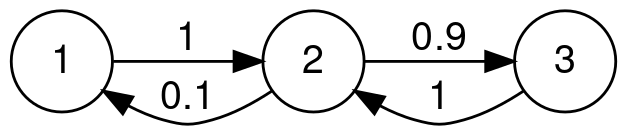
\includegraphics[width=6cm]{img/C3/ejemplo_diagrama_1.png}}
        \end{tabular}
        \end{tabular}
        $$

        En este caso, la cadena sería irreducible.
        \item\label{ej:diagramas-2} Supongamos ahora que la matriz y el diagrama son:
        $$
        \begin{tabular}{cc}
        \centering{\begin{tabular}{c}
            $P = \begin{pmatrix}
                0.5 & 0.3 & 0.2 \\
                0 & 1 & 0 \\
                0.5 & 0 & 0.5
            \end{pmatrix}
            $ \end{tabular}}&
        \begin{tabular}{c}
        \centering{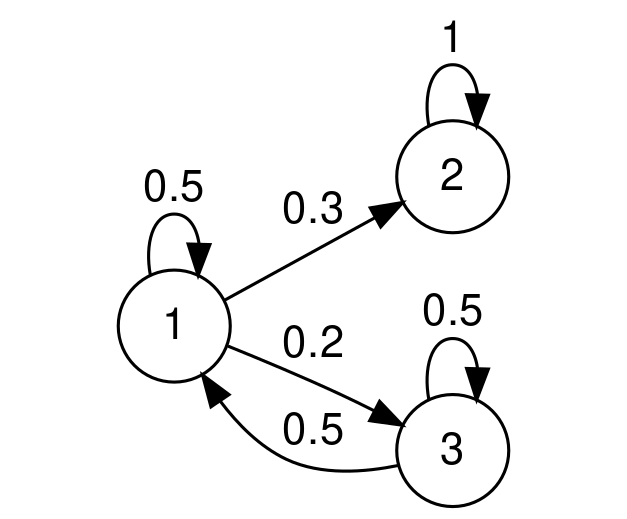
\includegraphics[width=5cm]{img/C3/ejemplo_diagrama_2.png}}
        \end{tabular}
        \end{tabular}
        $$
        % http://magjac.com/graphviz-visual-editor/

        Fijémonos que, aunque el estado $2$ es accesible desde todos los estados, ni el estado $1$ ni el $3$ son accesibles desde el $2$, lo cual impide que la cadena sea irreducible. Cuando un estado cumple esta propiedad se denomina estado \textit{absorbente}, término que definiremos formalmente más adelante.
    \end{enumerate}
    \label{ej:diagramas}
\end{ejemplo}

\cb{REVIEW añado algo sobre tema de matrices reducibles/irreducibles?}

Hemos clasificado los estados según su accesibilidad, pero fijémonos ahora en la posibilidad de revisitar o no un estado. En el ejemplo \ref{ej:diagramas}.\ref{ej:diagramas-1} es posible visitar cualquiera de los tres estados cada dos transiciones, mientras que en el ejemplo \ref{ej:diagramas}.\ref{ej:diagramas-2} es posible mantenerse en cualquiera de los tres estados iteración tras iteración. Sobre esta noción insiste la siguiente definición.

\begin{definicion}[Estado periódico, aperiódico y absorbente]
    \label{def:estado-periodico}
    Un estado $i$ es \textbf{periódico} de periodo $d_i$ si la cadena puede regresar a $i$ en pasos múltiplos de $d_i$. Si $d_i=1$, decimos que el estado $i$ es \textbf{aperiódico}. Si ningún estado de la cadena es accesible desde el estado $i$ (\textit{i.e.} $p_{ii}=1$), entonces el estado $i$ se denomina \textbf{absorbente}.
\end{definicion}

\begin{observacion}
    Si el estado $j$ es comunicante con un estado periódico, entonces $j$ es periódico.
\end{observacion}

Podemos extender esta definición a la cadena de Markov completa:

\begin{definicion}[Cadena de Markov periódica y aperiódica]
    Sea $\{X_n,n\geq 0\}$ una cadena de Markov homogénea, irreducible sobre un espacio de estados $S=\{1,\dots,N\}$. Sea $d$ el mayor número entero tal que, 
    \begin{equation}
        \label{eq:cond-periodica}
        p_{ii}^{(n)}>0 \Rightarrow d|n, \ \ \ \forall i\in S.
    \end{equation}
    Si $d>1$, la cadena de Markov es \textbf{periódica}, si $d=1$ es \textbf{aperiódica}.
\end{definicion}
Nótese que una cadena periódica puede volver a su estado inicial en $d,2d,3d,\dots$ transiciones. Lo interesante de esta definición y de que únicamente se aplique a cadenas irreducibles es que basta con hallar el mayor periodo $d_i$ (según la definición \ref{def:estado-periodico}) común a todos los estados, de forma que la irreducibilidad de la cadena garantiza que ese valor $d$ es válido para todos los estados. Por otro lado, si $p_{ii}>0$ para algún estado $i\in S$ en una cadena irreducible, necesariamente $d=1$ y la cadena es aperiódica.

\begin{observacion}
    La periodicidad también es fácil de consultar en los diagramas. Basta con definir un ciclo que empiece y termine en cada uno de los nodos. Entonces $d$ es el máximo común divisor de las longitudes de estos ciclos.
\end{observacion}

Así, la cadena del ejemplo \ref{ej:diagramas}.\ref{ej:diagramas-1} es periódica con $d=2$. Sin embargo, no podemos plantearnos la periodicidad de la cadena del ejemplo \ref{ej:diagramas}.\ref{ej:diagramas-2}, ya que ésta no es irreducible.

\cb{REVIEW Incluyo tema de estados absorbentes y transitorios?}

\subsection{Teoremas límite}

Una vez introducida la terminología principal de estados y cadenas, podemos estudiar la existencia y unicidad de una distribución límite. En primer lugar, vamos a asumir que existe al menos una distribución de probabilidad a la cual converge la distribución de $X_n$.

\begin{definicion}
    Llamamos \textbf{distribución límite} a la función masa de probabilidad a la cual converge la fmp de $X_n$ cuando $n$ tiende a infinito. Denotamos esta fmp como
    \begin{equation}
        \label{eq:distr-limite}
        \pi = (\pi_1,\dots,\pi_N)   ,
    \end{equation}
    donde $\pi_j=\displaystyle\lim_{n\rightarrow\infty} P[X_n=j], \ \ \ j\in S$.
\end{definicion}

Si asumimos la existencia de una distribución límite, esta debe cumplir ciertas propiedades.

\begin{proposicion}
    \label{prop:condiciones-limite}
    Si una cadena de Markov $\{X_n,n\geq 0\}$ admite una distribución límite $\pi$, entonces ésta verifica las siguientes propiedades:
    \begin{equation}
        \label{eq:condiciones-limite-1}
        \pi_j = \sum_{i=1}^N \pi_i p_{ij},\ \forall j\in S \ \ \ \ 
    \end{equation}
    \begin{equation}
        \label{eq:condiciones-limite-2}
        \sum_{j=1}^N \pi_j =1 \ \ \ \ 
    \end{equation}
    
\end{proposicion}
\begin{proof}
    Aplicando el teorema de la probabilidad total y el teorema de la probabilidad condicionada, tenemos que
    \begin{equation}
        \label{eq:prob-total-cond}
        P[X_{n+1}=j]=\sum_{i=1}^N P[X_n=i]p_{ij}, \ \ \ \forall j\in S.
    \end{equation}
    Si tomamos límite en ambos miembros de la igualdad cuando $n\rightarrow\infty$ y asumimos la existencia de esta distribución límite obtenemos la igualdad (1). La igualdad (2) se asume de la representación de $\pi$ como una función masa de probabilidad.
\end{proof}

La ecuación (\ref{eq:condiciones-limite-1}) también se escribe en forma matricial como 
\begin{equation}
    \label{eq:balance}
    \pi =\pi\cdot P.
\end{equation} 

Esta ecuación matricial puede resolverse, y si normalizamos el vector obtenido de forma que la suma de sus componentes resulte $1$, obtenemos un vector que denominaremos $\pi^*$. Supongamos ahora que $a^{(0)} = \pi^*$. Entonces, aplicando que es solución de (\ref{eq:balance}), $a^{(1)} = \pi^*\cdot P  = \pi^*$, $a^{(2)} = \pi^*\cdot P^2 = (\pi^* \cdot P) P = \pi^* \cdot P = \pi^*$, \dots, $a^{(n)}=\pi^*$. Es decir, la distribución de $X_n$, representada por el vector $a^{(n)}$, es la misma siempre independientemente de $n$ e igual a $\pi^*$. Es lo que en adelante denominaremos distribución estacionaria.

\begin{definicion}[Distribución estacionaria]
    \label{def:estacionaria}
    Una función masa de probabilidad dada por un vector fila $\pi^* =(\pi_1^*,\dots,\pi_N^*)$, se denomina \textbf{distribución estacionaria} de una cadena de Markov si
    \begin{equation}
        P[X_0=i]=\pi_i^* \ \ \forall i\in S \Rightarrow P[X_n=i]=\pi_i^*\ \ \forall i\in S, n\geq 0
    \end{equation}
    
\end{definicion}

Como vemos, las distribuciones límite y las distribuciones estacionarias guardan ambas una estrecha relación con las ecuaciones de la proposición \ref{prop:condiciones-limite}, y vemos que también la tendrán la existencia y unicidad de una y otra.

\begin{proposicion}
    Una función masa de probabilidad dada por un vector fila $\pi^* =(\pi_1^*,\dots,\pi_N^*)$ es una distribución estacionaria si, y solo si verifica las ecuaciones \eqref{eq:condiciones-limite-1} y \eqref{eq:condiciones-limite-2}.
\end{proposicion}
\begin{proof}
    Lo probaremos por doble implicación.
    \begin{itemize}
        \item[\fcolorbox{black}{white}{$\Rightarrow$}] Supongamos que $\pi^*$ cumple la propiedad de la definición \ref{def:estacionaria}. Si tomamos $n=0$ en (\ref{eq:prob-total-cond}) obtenemos
        $$
        P[X_{1}=j]=\sum_{i=1}^N P[X_0=i] p_{ij}, \ \ \ \forall j\in S.
        $$ 
        Pero como $P[X_0=j]=\pi_j^*$ y $P[X_{1}=j]=\pi_j^*$, sustituyendo obtenemos la igualdad (\ref{eq:condiciones-limite-1}). La ecuación (\ref{eq:condiciones-limite-2}) se deduce de que partimos de que $\pi^*$ es una función masa de probabilidad representada en un vector.
        \item[\fcolorbox{black}{white}{$\Leftarrow$}] Ahora asumimos que $\pi^*$ verifica las ecuaciones (\ref{eq:condiciones-limite-1}) y \eqref{eq:condiciones-limite-2}. Consideramos entonces que $P[X_0=j]=\pi_j^*, \ \ j\in S$. De nuevo, tomando $n=0$ en (\ref{eq:prob-total-cond}):
        $$
        P[X_{1}=j]=\sum_{i=1}^N P[X_0=i] p_{ij} = \sum_{i=1}^N \pi_i^* p_{ij} \underbrace{=}_{(\ref{eq:condiciones-limite-1})}\pi_j^*.
        $$
        Por lo que la fmp de $X_1$ es $\pi^*$. Si usamos repetidamente \eqref{eq:prob-total-cond} con distintos valores de $n$, deducimos que la fmp de $X_n$ es $\pi^*$ para cualquier $n\geq 0$. Esto es, $\pi^*$ es una distribución estacionaria.
    \end{itemize}
\end{proof}

El hecho de que tanto distribuciones límite como distribuciones estacionarias cumplan las mismas ecuaciones tiene una consecuencia sencilla de comprobar.

\begin{corolario}
    Si una cadena admite una distribución límite, entonces ésta es también una distribución estacionaria.
\end{corolario}

El concepto de cadena irreducible y el de distribución estacionaria confluyen en el siguiente resultado, cuya demostración omitiremos.

\begin{teorema}
    \label{th:teorema-estacionaria}
    Toda cadena de Markov finita e irreducible admite una única distribución estacionaria, \textit{i.e.}, la ecuación \eqref{eq:balance} tiene una única solución normalizada.
\end{teorema}

\begin{ejemplo}
    La distribución $\pi_1 = \left(0.05,\, 0.5,\, 0.45\right)$ es estacionaria para la cadena del ejemplo \ref{ej:diagramas}.\ref{ej:diagramas-1}.
\end{ejemplo}

Finalmente, presentaremos el último resultado de este capítulo, que es el que determina el comportamiento límite de las cadenas de Markov.

\begin{teorema}
    \label{th:teorema-limite}
    Toda cadena de Markov finita, irreducible y aperiódica admite una única distribución límite que es, además, estacionaria.
\end{teorema}

Con este último teorema, sumado a la última afirmación del enunciado del teorema \ref{th:teorema-estacionaria}, podemos conocer rápidamente el comportamiento límite de las cadenas de Markov que sean irreducibles y aperiódicas sin más que encontrar la única solución de las ecuaciones \eqref{eq:condiciones-limite-1} y \eqref{eq:condiciones-limite-2} (o la solución normalizada de la ecuación matricial \eqref{eq:balance}). 

El caso de cadenas de Markov reducibles y/o periódicas es más complejo. Por ejemplo, la distribución de $X_n$ puede converger a un ciclo de longitud $d$ si la cadena $\{X_n, n\geq 0\}$ es irreducible pero periódica con periodo $d$. O si es reducible, la distribución límite puede ser dependiente del estado inicial. Para un estudio más detallado de estos casos, así como la demostración de estos últimos teoremas, remitimos al lector a \cite[Ch. II, Sections 4.2 and 4.3]{Ross}.

\begin{ejemplo}
    Retomamos el ejemplo \ref{ej:cv} con la intención de predecir la población de cada provincia de la comunidad valenciana a largo plazo. Si nos fijamos en la matriz de transición podemos ver rápidamente que la cadena de Markov $\{X_n,n\geq 0\}$ es irreducible y aperiódica. Si resolvemos la ecuación $\pi=\pi \cdot P$, que es equivalente a resolver el sistema de ecuaciones 
    \begin{equation*}
        \pi_{1\times 3} (P-I_3)_{3\times 3} = 0_{1\times 3} 
    \end{equation*}
    obtenemos que su única solución normalizada es 
    \begin{equation*}
        \pi = \begin{pmatrix}
            0.3021799 & 0.1278348 & 0.5699852
        \end{pmatrix}
    \end{equation*}
    De esta forma, el modelo predice que la población a largo plazo de las provincias de la comunidad valenciana es la recogida en la tabla \ref{tab:poblacion-largo-plazo}.
    \begin{table}[h]
        \centering
        \begin{tabular}{cc}\hline
            \textbf{Provincia}  & \textbf{Población} \\ \hline\hline
            \textbf{Alicante} &  1 528 468 \\ \hline
            \textbf{Castellón} & 646 606.3 \\ \hline
            \textbf{Valencia} & 2 883 064 \\ \hline
        \end{tabular}
        \caption{Predicción de la población de las provincias de la C. Valenciana en el futuro}
        \label{tab:poblacion-largo-plazo}
    \end{table}
\end{ejemplo}

Para finalizar este capítulo, aclaramos que todos estos teoremas y definiciones tienen un análogo en el que se trabaja con columnas en lugar de con filas. Es decir, existe una manera distinta aunque equivalente de formular la teoría de las cadenas de Markov en la que las columnas de las matrices de transición suman $1$ (en lugar de las filas), las fmp se denotan con vectores columnas, las distribuciones transitorias se calculan multiplicando por la derecha un vector columna por la matriz de transición, etc. Es frecuente encontrar este enfoque en la literatura, aunque en nuestro caso se ha elegido éste por la intuición fácilmente recordable de que una probabilidad $p_{ij}$ sea la `probabilidad de ir desde el estado $i$ al estado $j$' por encima de que fuera la `probabilidad de llegar al estado $i$ desde el estado $j$'. 